
\subsection{Kompensation Störgröße Fahrzeug}
\label{headtracking_marker_subsec}

Bei einem stationären Fahrzeug genügt es, die Kopforientierung mittels \acs{IMU}-Daten der Brille zu bestimmen.
Die gesuchte Kopforientierung relativ zum Fahrzeug stimmt dabei mit der Kopforientierung bezüglich der Weltkoordinaten überein.
Sobald sich das Fahrzeug jedoch bewegt, wird die Schätzung der Kopforientierung verfälscht.
Fährt das Fahrzeug beispielsweise eine Kurve, so wird die von der IMU gemessene Drehung als Änderung des Yaw-Winkels der Kopforientierung interpretiert, obwohl der Fahrer in Bezug zum Fahrzeug weiterhin geradeaus blickt.

Eine weitere Störquelle stellt die Fahrzeugelektronik und die damit einhergehenden Änderungen des Magnetfelds dar.
Diese Störungen wirken sich negativ auf das zur Driftkorrektur eingesetzte Magnetometer aus (siehe Abschnitt \ref{headtracking_magnetometer_subsubsec}).

Zur Korrektur der Fehlschätzung aufgrund der genannten Einflüsse werden zwei Ansätze untersucht, die die Bestimmung der Kopforientierung relativ zum Fahrzeug stützen. Abb.~\ref{fig:tracking_ansaetze} zeigt die beiden Ansätze konzeptionell.

\begin{figure}[h]
  \centering
  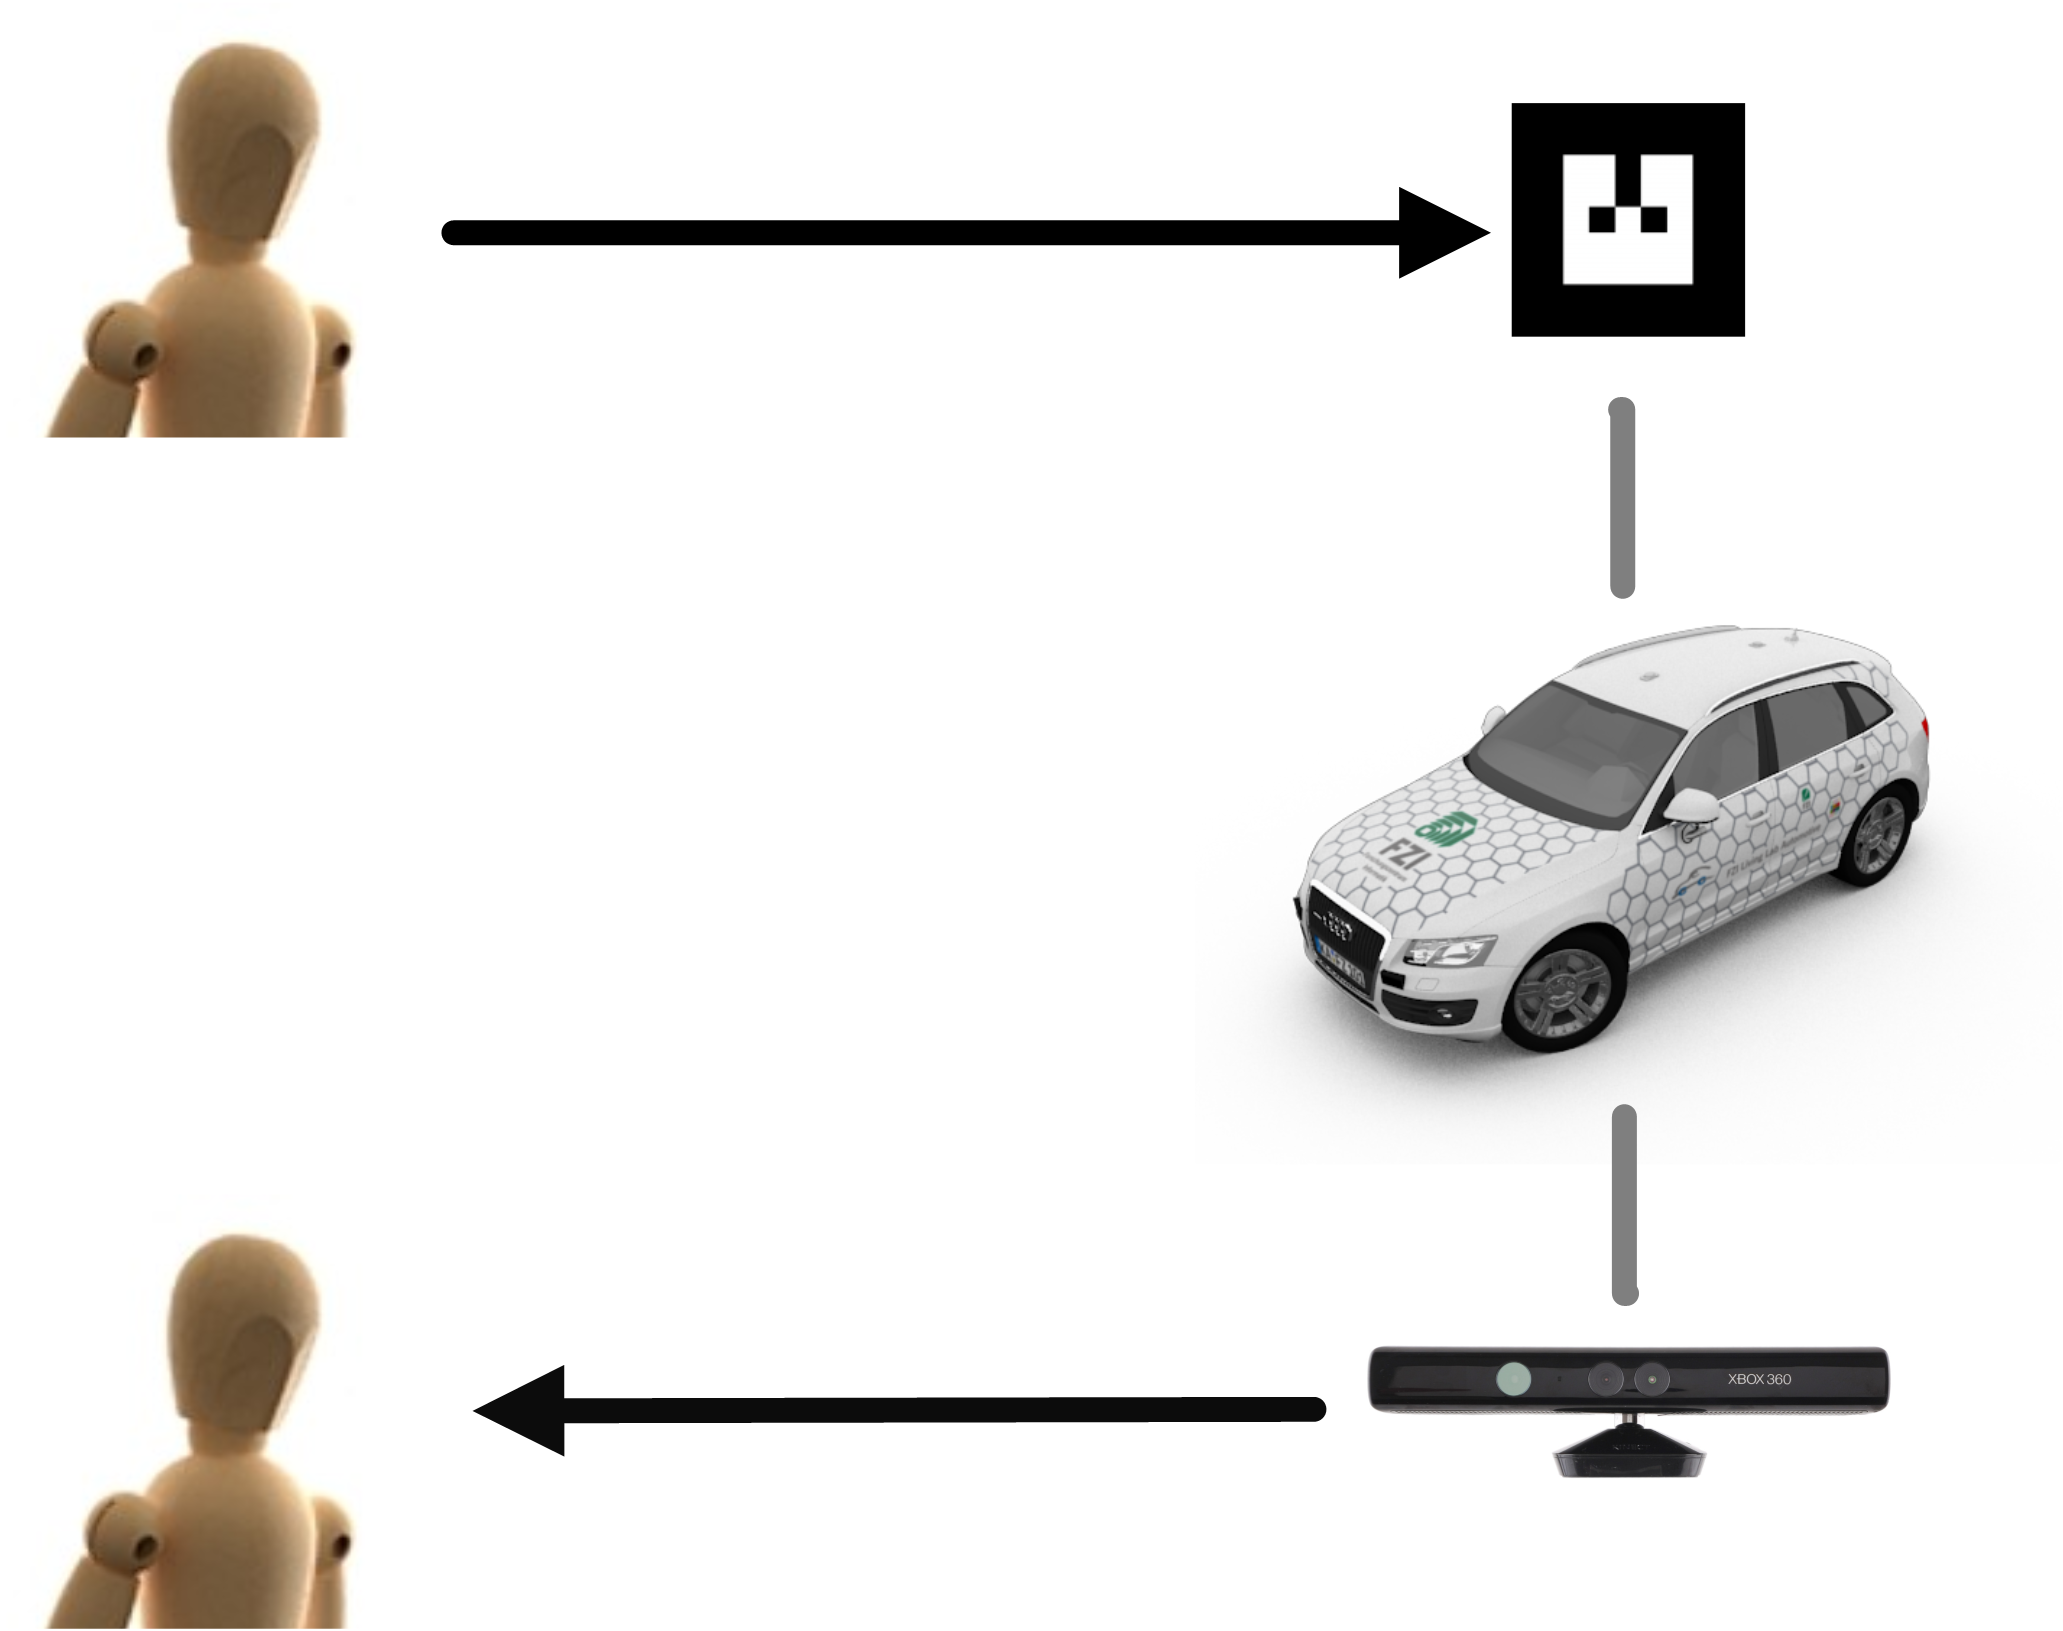
\includegraphics[width=0.4\textwidth]{Tracking_Ansaetze}
  \caption{Tracking-Ansätze: unten: Face-Tracking mit stationärer Kamera und bewegtem Kopf; oben: Marker-Tracking mit stationärem Marker und beweglicher Kamera }
  \label{fig:tracking_ansaetze}
\end{figure}


\subsubsection{Ansatz: Face-Tracking}
\label{headtracking_facetracking_subsubsec}

Die Idee beim Face-Tracking-Ansatz ist es, zu untersuchen, inwieweit die bestehende Hardware- und Software-Umgebung des CoCars für die Bestimmung der Kopforientierung verwendet werden kann.
Das Fahrzeug verfügt über eine fest installierte Kinect-Kamera, die auf den Fahrer ausgerichtet ist.
Für diese Kamera wurde am \ac{FZI} bereits ein Algorithmus zur Blickrichtungserkennung des Fahrers implementiert.
Der Algorithmus benutzt dafür ein Gesichtsmodell.
Das Gesichtsmodell berücksichtigt jedoch keine Brille.
Trägt der Fahrer eine Durchsichtbrille, ist ein Teil des Gesichts verdeckt.
Hierdurch wird die Erkennungsleistung stark beeinträchtigt.
Ein möglicher Ausweg ist das Einlernen des Gesichtsmodells mit Brille.
Jedoch ist die Spiegelung der von der Kinect verwendeten Infrarot-Strahlung an der Brille weiterhin problematisch.
Der Ansatz wird aus einem weiteren Grund nicht weiter verfolgt:
Die Verwendung von zusätzlicher Hardware schränkt die Wiederverwendbarkeit des Algorithmus zur Bestimmung der Kopforientierung ein.
Stattdessen fällt die Entscheidung auf einen Marker-Tracking-Ansatz, der alleine mit der Brillen-Hardware auskommt.


\subsubsection{Ansatz: Marker-Tracking}
\label{headtracking_markertracking_subsubsec}

Beim markerbasierten Tracking handelt es sich um ein optisches Trackingverfahren.
Dabei wird die Position und Orientierung eines speziellen Markers bestimmt, der im Kamerabild zu sehen ist.
Das Tracking übernimmt das \ac{ROS}-Paket \emph{ar\_track\_alvar}~\cite{ros_ar_track_alvar}, ein Wrapper für die Bibliothek \alvar.
Mit \alvar \ lassen sich Marker generieren, identifizieren sowie deren Posen im Kamerabild bestimmen - vorausgesetzt es wird eine kalibrierte Kamera verwendet.
Die Kamerakalibrierung kann mit dem \ac{ROS}-Paket \emph{camera\_calibration}~\cite{ros_camera_calibration} unter Verwendung eines Kalibrierschachbretts durchgeführt werden.
\alvar \ ermittelt die Pose des Markers in Bezug zum Kamerakoordinatensystem.
Für die Anwendung ist jedoch die Orientierung der Kamera von Interesse.
Sie wird als Kopforientierung interpretiert.
Wird der Marker als stationär angenommen, so kann die Inverse der von \alvar \ bestimmten Markerpose als Kamera- und somit als Kopfpose aufgefasst werden.
Abb.~\ref{fig:marker_in_vehicle_driver_view} zeigt den im Versuchsfahrzeug angebrachten Marker aus der Perspektive eines Fahrers.

\begin{figure}
  \centering
  \missingfigure{driver's view of marker}
  %\includegraphics[width=0.4\textwidth]{•}
  \caption{Marker im Fahrzeug aus Fahrerperspektive.}
  \label{fig:marker_in_vehicle_driver_view}
\end{figure}

Damit die berechnete Orientierung des Kopfes in Bezug zum Fahrzeug steht, muss der Marker im Fahrzeug kalibriert werden.
Die Kalibrierungsdaten setzen sich aus Position und Orientierung des Markers angegeben in Fahrzeugkoordinaten zusammen.
Für die Kalibrierung des Markers im Fahrzeug stehen drei Varianten zur Wahl:
\begin{enumerate}
 \item Manuelle Ausmessung im Versuchsfahrzeug.
 \item Schätzung anhand der durch \alvar \ ermittelten Markerpose.
 \item Schätzung anhand des 3D-Fahrzeugmodells.
\end{enumerate}

Mit der ersten Variante lassen sich die Kalibrierungsdaten am genauesten bestimmen.
Allerdings ist der Aufwand für die Ermittlung auch am größten.
Die erste Variante hat mit der zweiten Variante gemein, dass sie anfällig für Variationen der Markerpose im Fahrzeug sind. Wird der Marker beispielsweise aus- und wieder eingebaut, ist es schwierig, den Marker in die zuvor kalibrierte Pose zu bringen.
Folglich muss die Kalibrierung neu durchgeführt werden.
Die dritte Variante ist mit dem geringsten Zeitaufwand verbunden und bietet gleichzeitig die größte Flexibilität.
Das zur Verfügung stehende Fahrzeugmodell ist dabei auch hinreichend genau.
Mittels \emph{dynamic\_reconfigure}-Paket~\cite{ros_dynamic_reconfigure} kann eine grafische Benutzerschnittstelle zur Konfiguration der Posenparameter des Markermodells generiert werden.
So lassen sich die Parameter auch zur Laufzeit anpassen.
Unter Nutzung der rviz-Ansicht kann die konfigurierte Markerpose visuell überprüft werden.

Die Positionsangabe der von \alvar\ berechneten Markerpose wird in der Anwendung nicht genutzt, da die Kopfposition des Fahrers zur Vereinfachung als statisch angenommen wird.
Lediglich die Orientierung fließt in die folgende Fusion ein.

\subsubsection{Fusion IMU und Marker-Tracking}
\label{headracking_markerfusion_subsubsec}

